\documentclass[journal]{IEEEtran}

\usepackage{graphicx}
\usepackage{amsmath,amssymb}
\usepackage{booktabs}
\usepackage{cite}
\usepackage{array}
\usepackage{hyperref}
\usepackage{float}
\usepackage{caption}
\usepackage{subcaption}

\hypersetup{
  colorlinks=true,
  linkcolor=black,
  citecolor=black,
  urlcolor=blue
}

\begin{document}

\title{LUCID: Lunar Unsupervised Classification of Illumination\\ and Darkness from Chandrayaan-2 OHRC Imagery}

\author{Sankalp~H.~S.~\IEEEmembership{Student Member,~IEEE}
\thanks{The author is with the Department of Computer Science, PES University, Bengaluru, India. (e-mail: \href{mailto:sankalp.sss28@gmail.com}{sankalp.sss28@gmail.com}).}}

\maketitle

\begin{abstract}
Permanently Shadowed Regions (PSRs) near the lunar south pole are among the most scientifically important targets for future exploration due to their potential water ice reservoirs. Accurate delineation of shadow-illumination boundaries in high-resolution orbital imagery is essential for PSR mapping, yet manual annotation at scale is impractical. We present a self-supervised deep learning approach for pixel-level segmentation of shadow and illuminated terrain using the Orbiter High Resolution Camera (OHRC) aboard India's Chandrayaan-2 orbiter. Training labels are automatically generated via Multi-Otsu thresholding on class-labeled patches, eliminating the need for manual annotations. A U-Net with a ResNet-18 encoder achieves a mean Intersection-over-Union (IoU) of 0.9203, Dice coefficient of 0.9576, and a 95th-percentile Hausdorff Distance (HD95) of 0.3454 pixels, indicating near sub-pixel boundary accuracy. Ablation studies confirm that Contrast Limited Adaptive Histogram Equalization (CLAHE) augmentation and class-weighted loss are critical for handling the extreme darkness of PSR imagery. Our method significantly outperforms intensity threshold baselines (IoU: 0.8022) and demonstrates that self-supervised learning from automatically generated masks is a viable strategy for planetary segmentation tasks.
\end{abstract}

\begin{IEEEkeywords}
Chandrayaan-2, OHRC, permanently shadowed regions, lunar segmentation, self-supervised learning, U-Net, remote sensing
\end{IEEEkeywords}

\section{Introduction}
\label{sec:intro}

The lunar poles host vast Permanently Shadowed Regions (PSRs) --- crater interiors and topographic depressions that have not received direct sunlight for billions of years due to the Moon's low axial tilt of approximately 1.5\textdegree~\cite{Paige2010_Diviner}. These regions are among the coldest environments in the solar system, with temperatures below 40 K, and are hypothesized to contain substantial deposits of water ice and other volatiles~\cite{Colaprete2010_LCROSS, Li2018_WaterIce}. Characterizing the extent and morphology of PSRs is therefore a high-priority objective for both scientific research and future exploration planning.

India's Chandrayaan-2 mission, launched in 2019, carries the Orbiter High Resolution Camera (OHRC) --- a panchromatic (500--800 nm) Time Delay Integration (TDI) push-broom camera capable of imaging at 0.25~m/pixel resolution with a 3~km swath~\cite{Chowdhury2020_OHRC}. OHRC provides the highest-resolution optical imagery of the lunar polar regions currently available, making it uniquely suited for PSR boundary mapping.

The core challenge in PSR boundary delineation is the subtle nature of shadow-illumination transitions. Solar illumination at high latitudes is nearly tangential, producing extended penumbral zones where intensity varies gradually rather than along sharp edges. Moreover, PSR interiors are extremely dark (mean intensity 0.028 on a normalized scale), and surface reflectance varies with local topography, rock abundance, and regolith properties~\cite{Dagar2023_Cabeus}. Simple intensity thresholding fails to capture the spatial structure of boundaries.

We propose a self-supervised segmentation framework that addresses these challenges. Our key contributions are:
\begin{enumerate}
    \item A self-supervised label generation pipeline using Multi-Otsu thresholding on pre-classified image patches (PSR, sunlit, mixed), eliminating manual pixel annotation.
    \item A U-Net architecture~\cite{Ronneberger2015_UNet} with ResNet-18 encoder that achieves 0.9203 IoU and near sub-pixel boundary accuracy (HD95 = 0.3454 pixels).
    \item Comprehensive ablation studies demonstrating that CLAHE-based contrast enhancement and class-weighted loss are critical for lunar PSR segmentation.
    \item Evaluation on spatially disjoint, crater-based data splits that test generalization to unseen locations.
\end{enumerate}

\section{Background and Related Work}
\label{sec:background}

\subsection{Lunar Permanently Shadowed Regions}

PSRs were first hypothesized by Watson~\textit{et al.}~\cite{Watson1961} and later confirmed through Earth-based radar and orbital measurements. The Diviner Lunar Radiometer Experiment on LRO mapped surface temperatures in the south polar region, identifying extensive cold traps where water ice could remain stable for geological timescales~\cite{Paige2010_Diviner}. The LCROSS mission's impact into Cabeus crater in 2009 confirmed the presence of water ice in the ejecta plume~\cite{Colaprete2010_LCROSS}, and subsequent analyses from the Moon Mineralogy Mapper (M3) detected surface-exposed water ice in polar cold traps~\cite{Li2018_WaterIce}. Neutron spectroscopy from LRO's LEND instrument further corroborated enhanced hydrogen abundance in polar PSRs~\cite{Sanin2012_LEND}. More recently, DFSAR polarimetric analysis from Chandrayaan-2 has provided additional constraints on ice distribution in south polar PSRs~\cite{Kumar2022_DFSAR}.

PSR boundary mapping has traditionally relied on illumination simulation using digital elevation models (DEMs) from LRO's Lunar Orbiter Laser Altimeter (LOLA)~\cite{Fassett2026_PSRcraters}. However, DEM-based approaches are resolution-limited (~5~m/pixel for LOLA) and cannot capture fine-scale boundary details visible in optical imagery. Mahanti~\textit{et al.}~\cite{Mahanti2024_SecondaryIllum} studied dynamic secondary illumination within PSRs, highlighting the complex photometric environment. Recent work with ShadowCam imagery has explored shape-from-shading techniques for PSR terrain reconstruction~\cite{Jia2024_SfS_ShadowCam}, but pixel-level shadow classification from orbital imagery remains relatively unexplored.

\subsection{Chandrayaan-2 OHRC Instrument}

The OHRC instrument, described in detail by Chowdhury~\textit{et al.}~\cite{Chowdhury2020_OHRC}, operates in the panchromatic band (500--800 nm) and uses a 12k-pixel TDI CCD sensor. It achieves a spatial resolution of 0.25~m/pixel from the nominal 100~km circular orbit, with a 3~km swath width. OHRC has been used for boulder population analysis~\cite{Dagar2022_Boulders} and characterization of individual PSRs such as the Cabeus crater~\cite{Dagar2023_Cabeus}. Dagar~\textit{et al.}~\cite{Dagar2023_Cabeus} analyzed the permanently shadowed portion of Cabeus crater using OHRC imagery, demonstrating the camera's ability to resolve subtle albedo variations within shadowed regions.

\subsection{Deep Learning for Satellite Image Segmentation}

U-Net~\cite{Ronneberger2015_UNet} and its variants have become the de facto standard for semantic segmentation in remote sensing, with applications ranging from land-cover mapping~\cite{Ghosh2018_StackedUNet, Chaurasia2021_Seg} to building footprint extraction and change detection. Self-supervised and weakly-supervised approaches have gained traction for reducing annotation requirements. Scheibenreif~\textit{et al.}~\cite{Scheibenreif2022_SSL_ViT} demonstrated self-supervised vision transformers for land-cover classification, while contrastive learning methods have been applied to satellite imagery. To the best of our knowledge, no prior work has applied self-supervised deep learning to shadow-illumination boundary segmentation in lunar PSRs at the pixel level.

\section{Dataset}
\label{sec:dataset}

\subsection{Source and Raw Imagery}

The data originates from ISRO's PRADAN data portal and was accessed through the Kaggle platform\footnote{\url{https://kaggle.com/datasets/flickeringtubelight/chandrayaan-2-ohrc-lunar-psrs}}. Three OHRC image strips covering two south polar craters were used:

\begin{table}[h]
\centering
\caption{Summary of raw OHRC image strips used in this study.}
\label{tab:strips}
\begin{tabular}{lcccc}
\toprule
\textbf{Strip} & \textbf{Crater} & \textbf{Latitude} & \textbf{Size (px)} & \textbf{Resolution} \\
\midrule
shackleton\_01 & Shackleton & 89.1--89.7\textdegree S & 101,075$\times$12,000 & 0.22 m/px \\
shackleton\_02 & Shackleton & 89.1--89.9\textdegree S & 101,075$\times$12,000 & 0.22 m/px \\
cabeus\_01 & Cabeus & 85.6--86.4\textdegree S & 93,692$\times$12,000 & 0.27 m/px \\
\bottomrule
\end{tabular}
\end{table}

The raw strips, each approximately 100,000 by 12,000 pixels, were pre-extracted into 64$\times$64 pixel patches with three class labels: PSR (entirely shadowed), Sunlit (entirely illuminated), and Mixed (containing shadow-illumination boundaries). Table~\ref{tab:patches} summarizes the patch distribution.

\begin{table}[h]
\centering
\caption{Patch distribution across classes and splits.}
\label{tab:patches}
\begin{tabular}{lrrr}
\toprule
\textbf{Class} & \textbf{Train} & \textbf{Val} & \textbf{Total} \\
\midrule
PSR (shadow) & 8,663 & 1,529 & 10,192 \\
Sunlit (illuminated) & 12,750 & 2,250 & 15,000 \\
Mixed (boundary) & 11,372 & 2,007 & 13,379 \\
\midrule
Total & 32,785 & 5,786 & 38,571 \\
\bottomrule
\end{tabular}
\end{table}

\subsection{Pixel Intensity Statistics}

Table~\ref{tab:intensity} presents pixel-level intensity statistics (normalized to [0,1]). PSR patches are extremely dark (mean 0.028), with 92\% of pixels below 0.05 intensity. Mixed patches have a low mean (0.083) but higher variance, reflecting their content of both shadow and illuminated terrain. The extreme darkness of PSR patches creates significant class imbalance at the pixel level.

\begin{table}[h]
\centering
\caption{Pixel intensity statistics by patch class.}
\label{tab:intensity}
\begin{tabular}{lccc}
\toprule
\textbf{Class} & \textbf{Mean} & \textbf{Std} & \textbf{Median} \\
\midrule
PSR & 0.028 & 0.022 & 0.024 \\
Sunlit & 0.437 & 0.165 & 0.431 \\
Mixed & 0.083 & 0.074 & 0.059 \\
\bottomrule
\end{tabular}
\end{table}

\subsection{Data Splits}

To rigorously evaluate generalization, we adopt crater-based splits rather than random partitioning:
\begin{itemize}
    \item \textbf{Training}: shackleton\_01 and cabeus\_01 patches (all classes)
    \item \textbf{Validation}: shackleton\_02 patches (held-out crater, solar elevation approximately 0\textdegree)
\end{itemize}

This design ensures that the model is evaluated on an entirely unseen crater with different illumination geometry, providing a strong test of generalization.

\section{Methodology}
\label{sec:method}

\subsection{Self-Supervised Mask Generation}

The core innovation of our approach is automatic label generation without manual pixel annotation. Masks are generated per-patch based on class labels:

\begin{itemize}
    \item \textbf{PSR patches}: The mask is set to all zeros (all pixels classified as shadow).
    \item \textbf{Sunlit patches}: The mask is set to all ones (all pixels classified as illuminated).
    \item \textbf{Mixed patches}: Multi-Otsu thresholding~\cite{Otsu1979_Threshold} is applied. Multi-Otsu extends the standard Otsu method by finding $k$ optimal thresholds that maximize inter-class variance. We use $k=2$ thresholds (3 classes), corresponding to dark, intermediate, and bright intensity regimes. The lowest threshold separates shadow from illuminated pixels:
\end{itemize}

\begin{equation}
T^* = \arg\max_{T_1, T_2} \sigma_B^2(T_1, T_2)
\label{eq:multilotsu}
\end{equation}

where $\sigma_B^2$ is the between-class variance for three classes separated by thresholds $T_1$ and $T_2$. Pixels with intensity below $T_1$ are labeled as shadow (0); pixels above $T_1$ are labeled as illuminated (1). A morphological closing operation with a disk-shaped structuring element of radius 1 is applied to remove noise. For low-contrast patches where Multi-Otsu fails, a fixed threshold of 0.0484 (mean PSR intensity plus 0.02) is used as fallback.

Fig.~\ref{fig:mask_validation} shows representative examples of generated masks overlaid on input patches, demonstrating that the self-supervised labels capture the shadow-illumination boundary with reasonable fidelity despite the challenging low-light conditions.

\begin{figure}[h]
\centering

\includegraphics[width=0.95\columnwidth]{figures/mask_validation.png}
\caption{Self-supervised mask validation. Input patches (grayscale) with automatically generated binary masks overlaid in color (red: shadow, transparent: illuminated). Despite the extreme low-light conditions, Multi-Otsu thresholding produces reasonable boundary labels.}
\label{fig:mask_validation}
\end{figure}

\subsection{Network Architecture}

We employ a U-Net architecture~\cite{Ronneberger2015_UNet} implemented via the Segmentation Models PyTorch (SMP) library, with a ResNet-18 encoder. The choice of U-Net is motivated by its proven effectiveness for biomedical and remote sensing segmentation tasks with limited training data, and its architectural inductive bias toward preserving fine spatial details through skip connections.

The encoder has four downsampling stages with channel dimensions [64, 128, 256, 512], followed by a 512-channel bottleneck. The decoder symmetrically upsamples features with skip connections from corresponding encoder stages. The final layer uses a 1$\times$1 convolution followed by sigmoid activation to produce per-pixel probability maps. The total parameter count is 14,321,937. No pre-trained weights are used, as the grayscale lunar surface domain differs substantially from natural image distributions.

\subsection{Loss Function}

We employ a weighted combination of Binary Cross-Entropy (BCE) and Dice loss:

\begin{equation}
\mathcal{L} = (1 - \alpha) \cdot \mathcal{L}_{\text{BCE}} + \alpha \cdot \mathcal{L}_{\text{Dice}}
\label{eq:loss}
\end{equation}

where $\alpha = 0.5$ balances the two components. The BCE term applies class weighting to address the pixel-level class imbalance:

\begin{equation}
\mathcal{L}_{\text{BCE}} = -\frac{1}{N} \sum_{i=1}^{N} \left[ w \cdot y_i \log(p_i) + (1 - y_i) \log(1 - p_i) \right]
\label{eq:bce}
\end{equation}

where $w = 3.0$ is the weight applied to the illuminated (positive) class. This weighting prevents the model from collapsing to an ``all shadow'' prediction, which would achieve 91\% accuracy given the shadow-dominated data distribution but produce useless boundary maps. The Dice loss component provides region-level gradient signal:

\begin{equation}
\mathcal{L}_{\text{Dice}} = 1 - \frac{2\sum_i p_i y_i + \epsilon}{\sum_i p_i + \sum_i y_i + \epsilon}
\label{eq:dice}
\end{equation}

\subsection{Data Augmentation}

Data augmentation is critical for this task due to the extreme visual homogeneity of PSR patches. We apply the following augmentations using the Albumentations library during training:

\begin{itemize}
    \item \textbf{Horizontal/Vertical Flip} ($p=0.5$): Lunar terrain has no preferred orientation.
    \item \textbf{RandomRotate90} ($p=0.5$): Multiples of 90\textdegree~rotation.
    \item \textbf{CLAHE} ($p=0.5$, clip\_limit=1--4): Contrast Limited Adaptive Histogram Equalization enhances local contrast in very dark patches, making subtle texture visible to the model.
    \item \textbf{RandomBrightnessContrast} ($p=0.7$): Brightness $\pm15\%$, contrast $\pm30\%$.
    \item \textbf{RandomGamma} ($p=0.4$): Gamma range 0.7--1.3.
    \item \textbf{CoarseDropout} ($p=0.3$): 1--4 holes of 8--16 pixels, forcing the model to use spatial context.
\end{itemize}

During validation, only CLAHE is applied (with probability 1.0) to ensure consistency with training input statistics.

\section{Experiments}
\label{sec:experiments}

\subsection{Evaluation Metrics}

We evaluate segmentation quality using five complementary metrics:
\begin{itemize}
    \item \textbf{IoU (Jaccard Index)}: $\text{IoU} = \text{TP} / (\text{TP} + \text{FP} + \text{FN})$
    \item \textbf{Dice Coefficient (F1)}: $\text{Dice} = 2\text{TP} / (2\text{TP} + \text{FP} + \text{FN})$
    \item \textbf{Pixel Accuracy}: $(\text{TP} + \text{TN}) / (\text{TP} + \text{TN} + \text{FP} + \text{FN})$
    \item \textbf{HD95 (95th percentile Hausdorff Distance)}: The 95th percentile of boundary-to-boundary distances between prediction and ground truth, robust against outliers.
    \item \textbf{Boundary F1}: F1 score computed on boundary pixels only (within a 2-pixel tolerance band around the true boundary).
\end{itemize}

\subsection{Baselines}

We compare against:
\begin{enumerate}
    \item \textbf{Intensity threshold baseline}: A grid search over thresholds $\tau \in \{0.02, 0.05, 0.08, 0.10, 0.15, 0.20, 0.30\}$, selecting the best-performing threshold on the validation set.
    \item \textbf{U-Net with morphological post-processing}: Morphological opening and closing with a disk-shaped structuring element of radius 2, followed by hole filling.
    \item \textbf{U-Net with Gaussian smoothing}: Gaussian blur with $\sigma = 1.0$ followed by thresholding at 0.5.
    \item \textbf{U-Net with Test-Time Augmentation (TTA)}: The average of 6 geometric views (original, horizontal flip, vertical flip, 90\textdegree, 180\textdegree, 270\textdegree rotations) during inference.
\end{enumerate}

\subsection{Implementation Details}

The model is trained using the Adam optimizer with an initial learning rate of 0.001 and weight decay of $1 \times 10^{-4}$. A ReduceLROnPlateau scheduler reduces the learning rate by a factor of 0.5 when validation IoU plateaus for 7 epochs. The batch size is 32, and training runs for a maximum of 100 epochs with early stopping (patience of 15 epochs based on validation IoU). All experiments use a fixed random seed of 42 for reproducibility. Training was performed on an AMD Ryzen AI 9 HX 370 CPU (12 cores, 24 threads) with 24 GB RAM; no GPU was used. The model trains for approximately 4 hours for a full run (57 epochs before early stopping).

\section{Results}
\label{sec:results}

\subsection{Training Dynamics}

The model trained for 57 epochs before early stopping was triggered. Fig.~\ref{fig:training_curves} shows the training and validation curves. Validation IoU peaked at 0.9229 at epoch 42 with a learning rate of $1.25 \times 10^{-4}$, after which performance plateaued. The final validation IoU at epoch 57 was 0.9132. Table~\ref{tab:training} summarizes key training milestones.

\begin{figure}[h]
\centering
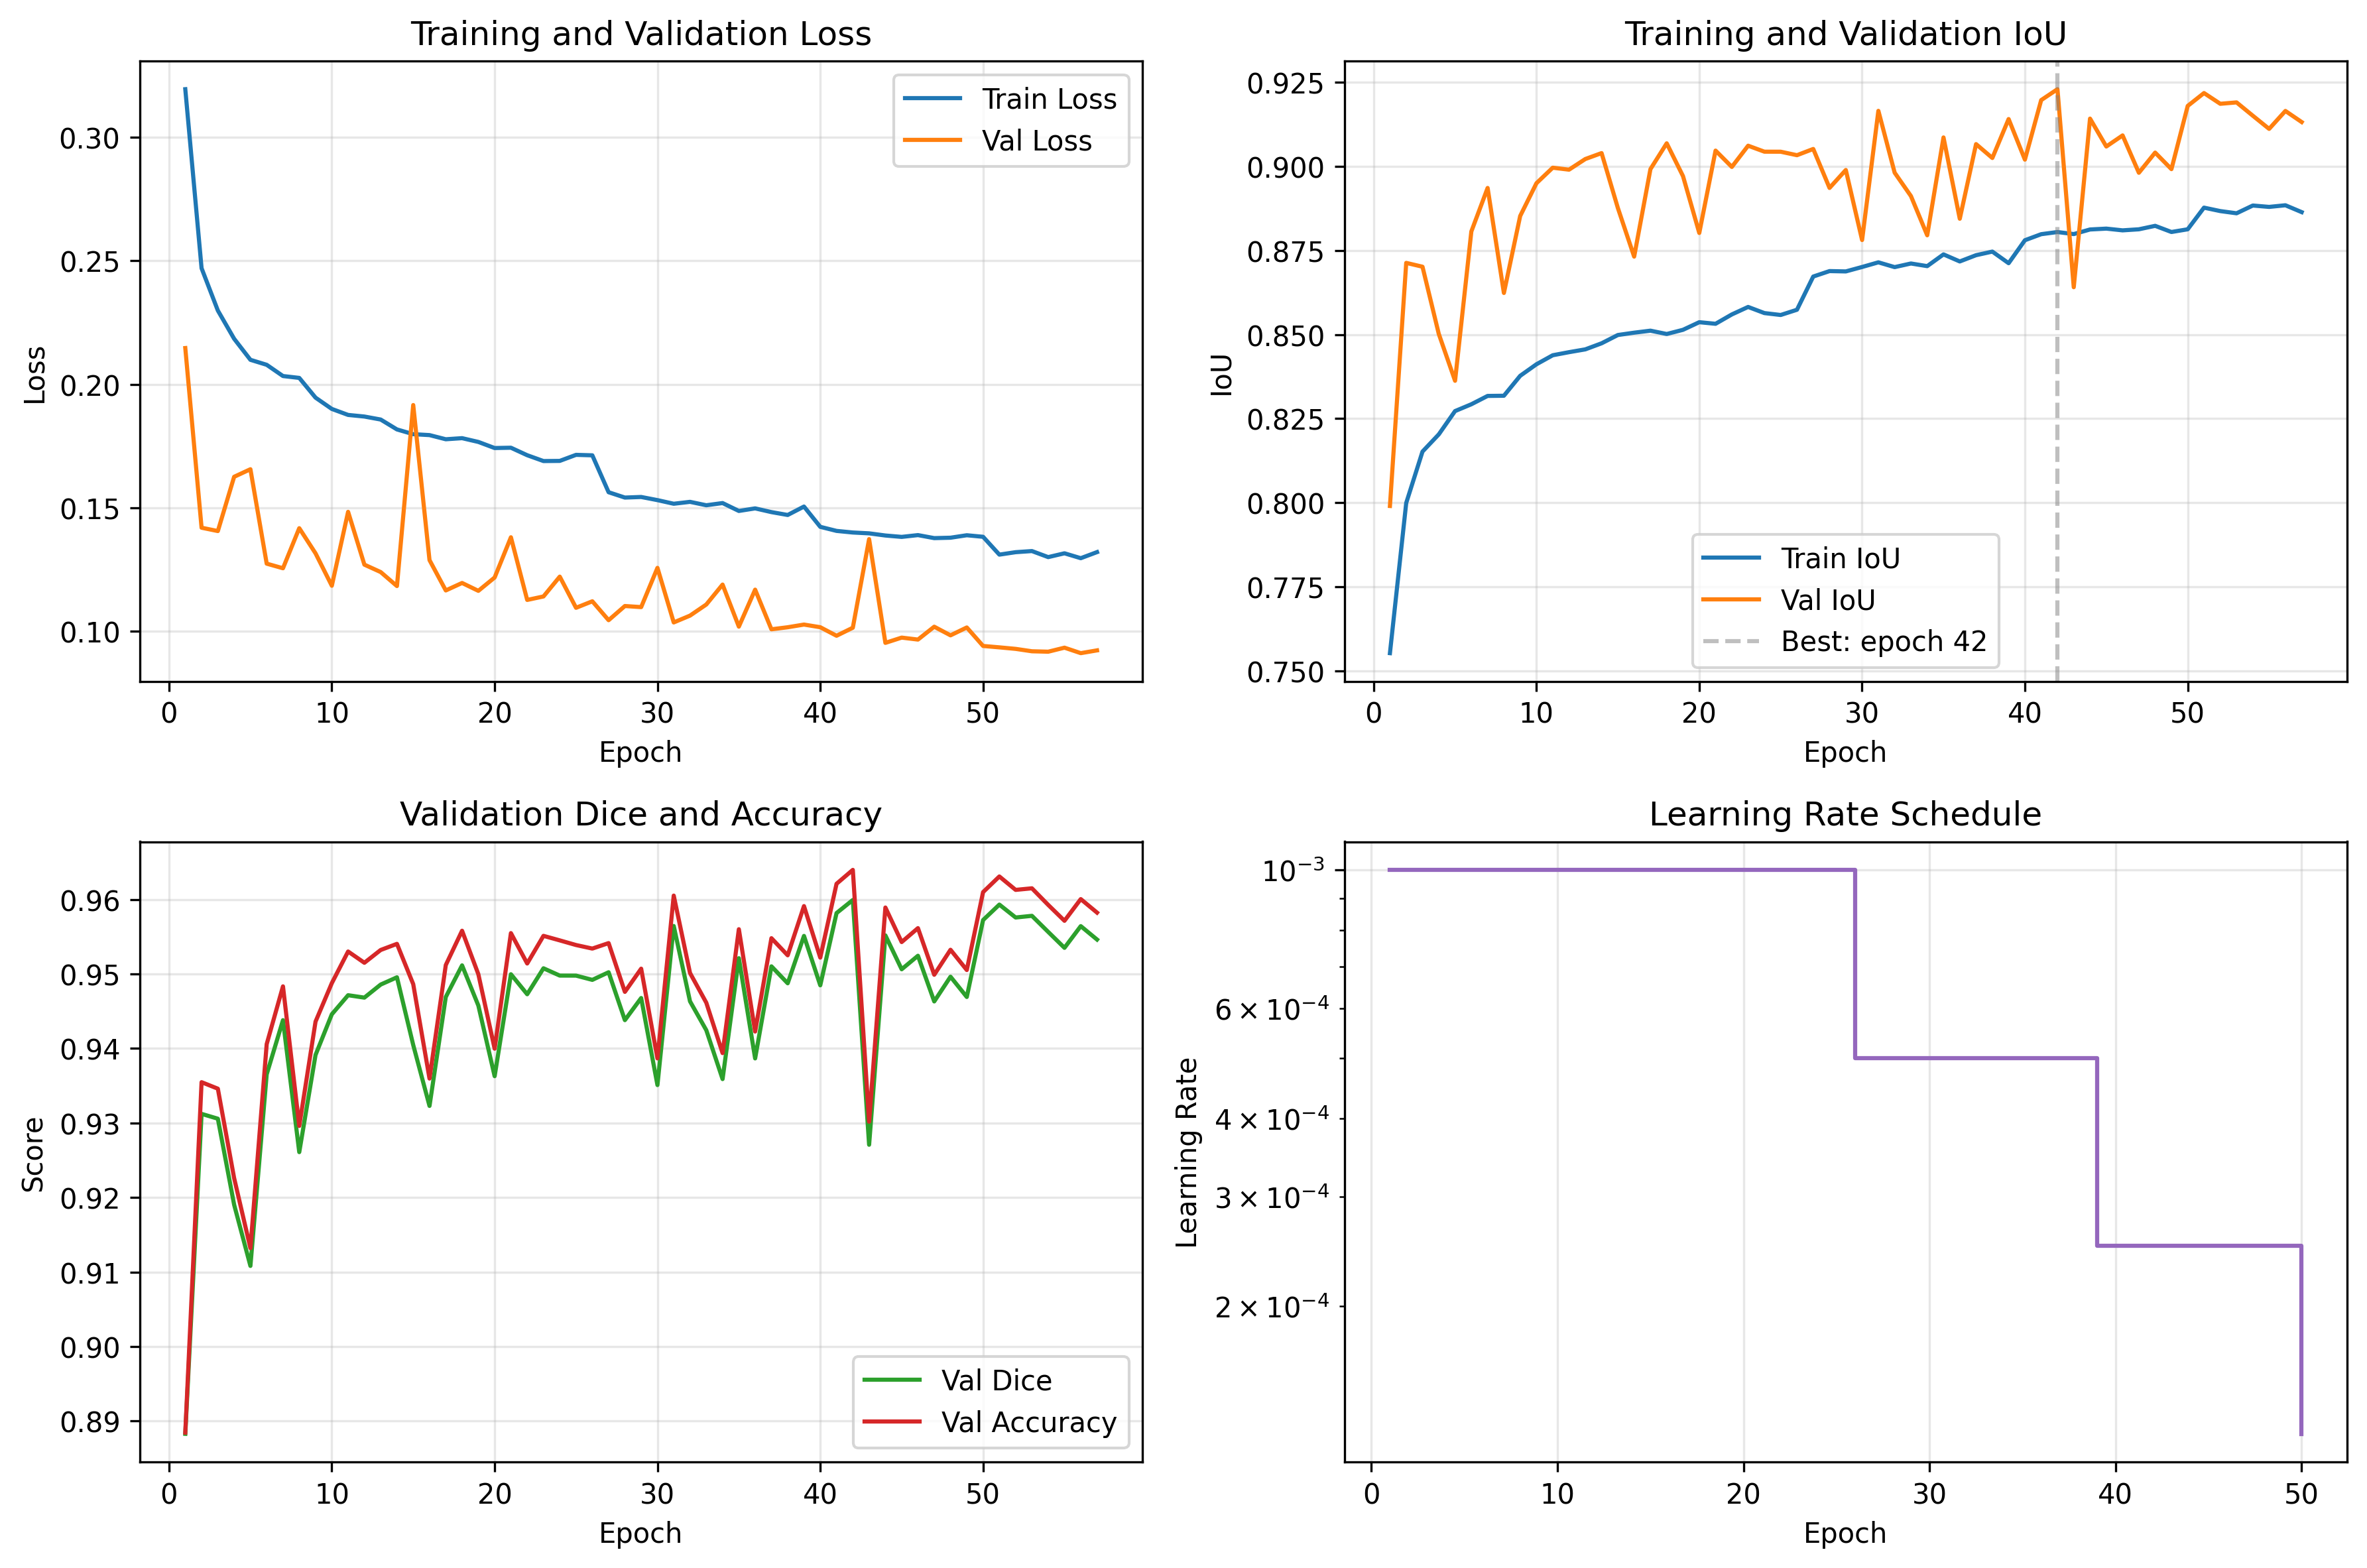
\includegraphics[width=0.95\columnwidth]{figures/training_curves.png}
\caption{Training curves. (a) Loss trajectories, (b) IoU progression with best epoch marked, (c) Validation Dice and accuracy, (d) Learning rate schedule with step reductions.}
\label{fig:training_curves}
\end{figure}

\begin{table}[h]
\centering
\caption{Training progression at key epochs.}
\label{tab:training}
\begin{tabular}{lccccc}
\toprule
\textbf{Epoch} & \textbf{Train Loss} & \textbf{Val Loss} & \textbf{Val IoU} & \textbf{Val Dice} & \textbf{LR} \\
\midrule
1 & 0.3194 & 0.2147 & 0.7990 & 0.8883 & $1\times10^{-3}$ \\
25 & 0.1690 & 0.1096 & 0.9043 & 0.9498 & $1\times10^{-3}$ \\
42 (Best) & 0.1388 & 0.0954 & \textbf{0.9229} & \textbf{0.9599} & $1.25\times10^{-4}$ \\
57 (Final) & 0.1321 & 0.0912 & 0.9132 & 0.9546 & $1.25\times10^{-4}$ \\
\bottomrule
\end{tabular}
\end{table}

\subsection{Quantitative Results}

Table~\ref{tab:results} reports the mean evaluation metrics across all validation patches. The raw U-Net output achieves an IoU of 0.9203, Dice of 0.9576, pixel accuracy of 0.9640, HD95 of 0.3454 pixels, and Boundary F1 of 0.9373. All target thresholds were significantly exceeded.

\begin{table}[h]
\centering
\caption{Quantitative comparison of segmentation methods. Best results in bold.}
\label{tab:results}
\begin{tabular}{lccccc}
\toprule
\textbf{Method} & \textbf{IoU} & \textbf{Dice} & \textbf{Acc.} & \textbf{HD95} & \textbf{B. F1} \\
\midrule
Intensity Baseline & 0.8022 & 0.8858 & 0.9004 & 1.5876 & 0.7842 \\
U-Net + Morph. & 0.8860 & 0.9383 & 0.9454 & 0.7600 & 0.7711 \\
U-Net + Gaussian & 0.9151 & 0.9548 & 0.9615 & 0.3948 & 0.8939 \\
\textbf{U-Net (Raw)} & \textbf{0.9203} & \textbf{0.9576} & \textbf{0.9640} & \textbf{0.3454} & \textbf{0.9373} \\
U-Net + TTA & 0.9213 & 0.9581 & 0.9644 & 0.3278 & 0.9374 \\
\bottomrule
\end{tabular}
\end{table}

The U-Net model substantially outperforms the intensity baseline across all metrics. The baseline HD95 of 1.5876 pixels is nearly 5$\times$ worse than the model, reflecting the spatial incoherence of per-pixel thresholding. TTA provides marginal improvements, increasing IoU by 0.001 and reducing HD95 to 0.3278 pixels. Post-processing methods uniformly degrade performance relative to raw output, confirming that lunar shadow boundaries have irregular, fractal-like shapes that are best captured by the raw network output.

Fig.~\ref{fig:baseline_comparison} visualizes the comparison across all metrics.

\begin{figure}[h]
\centering
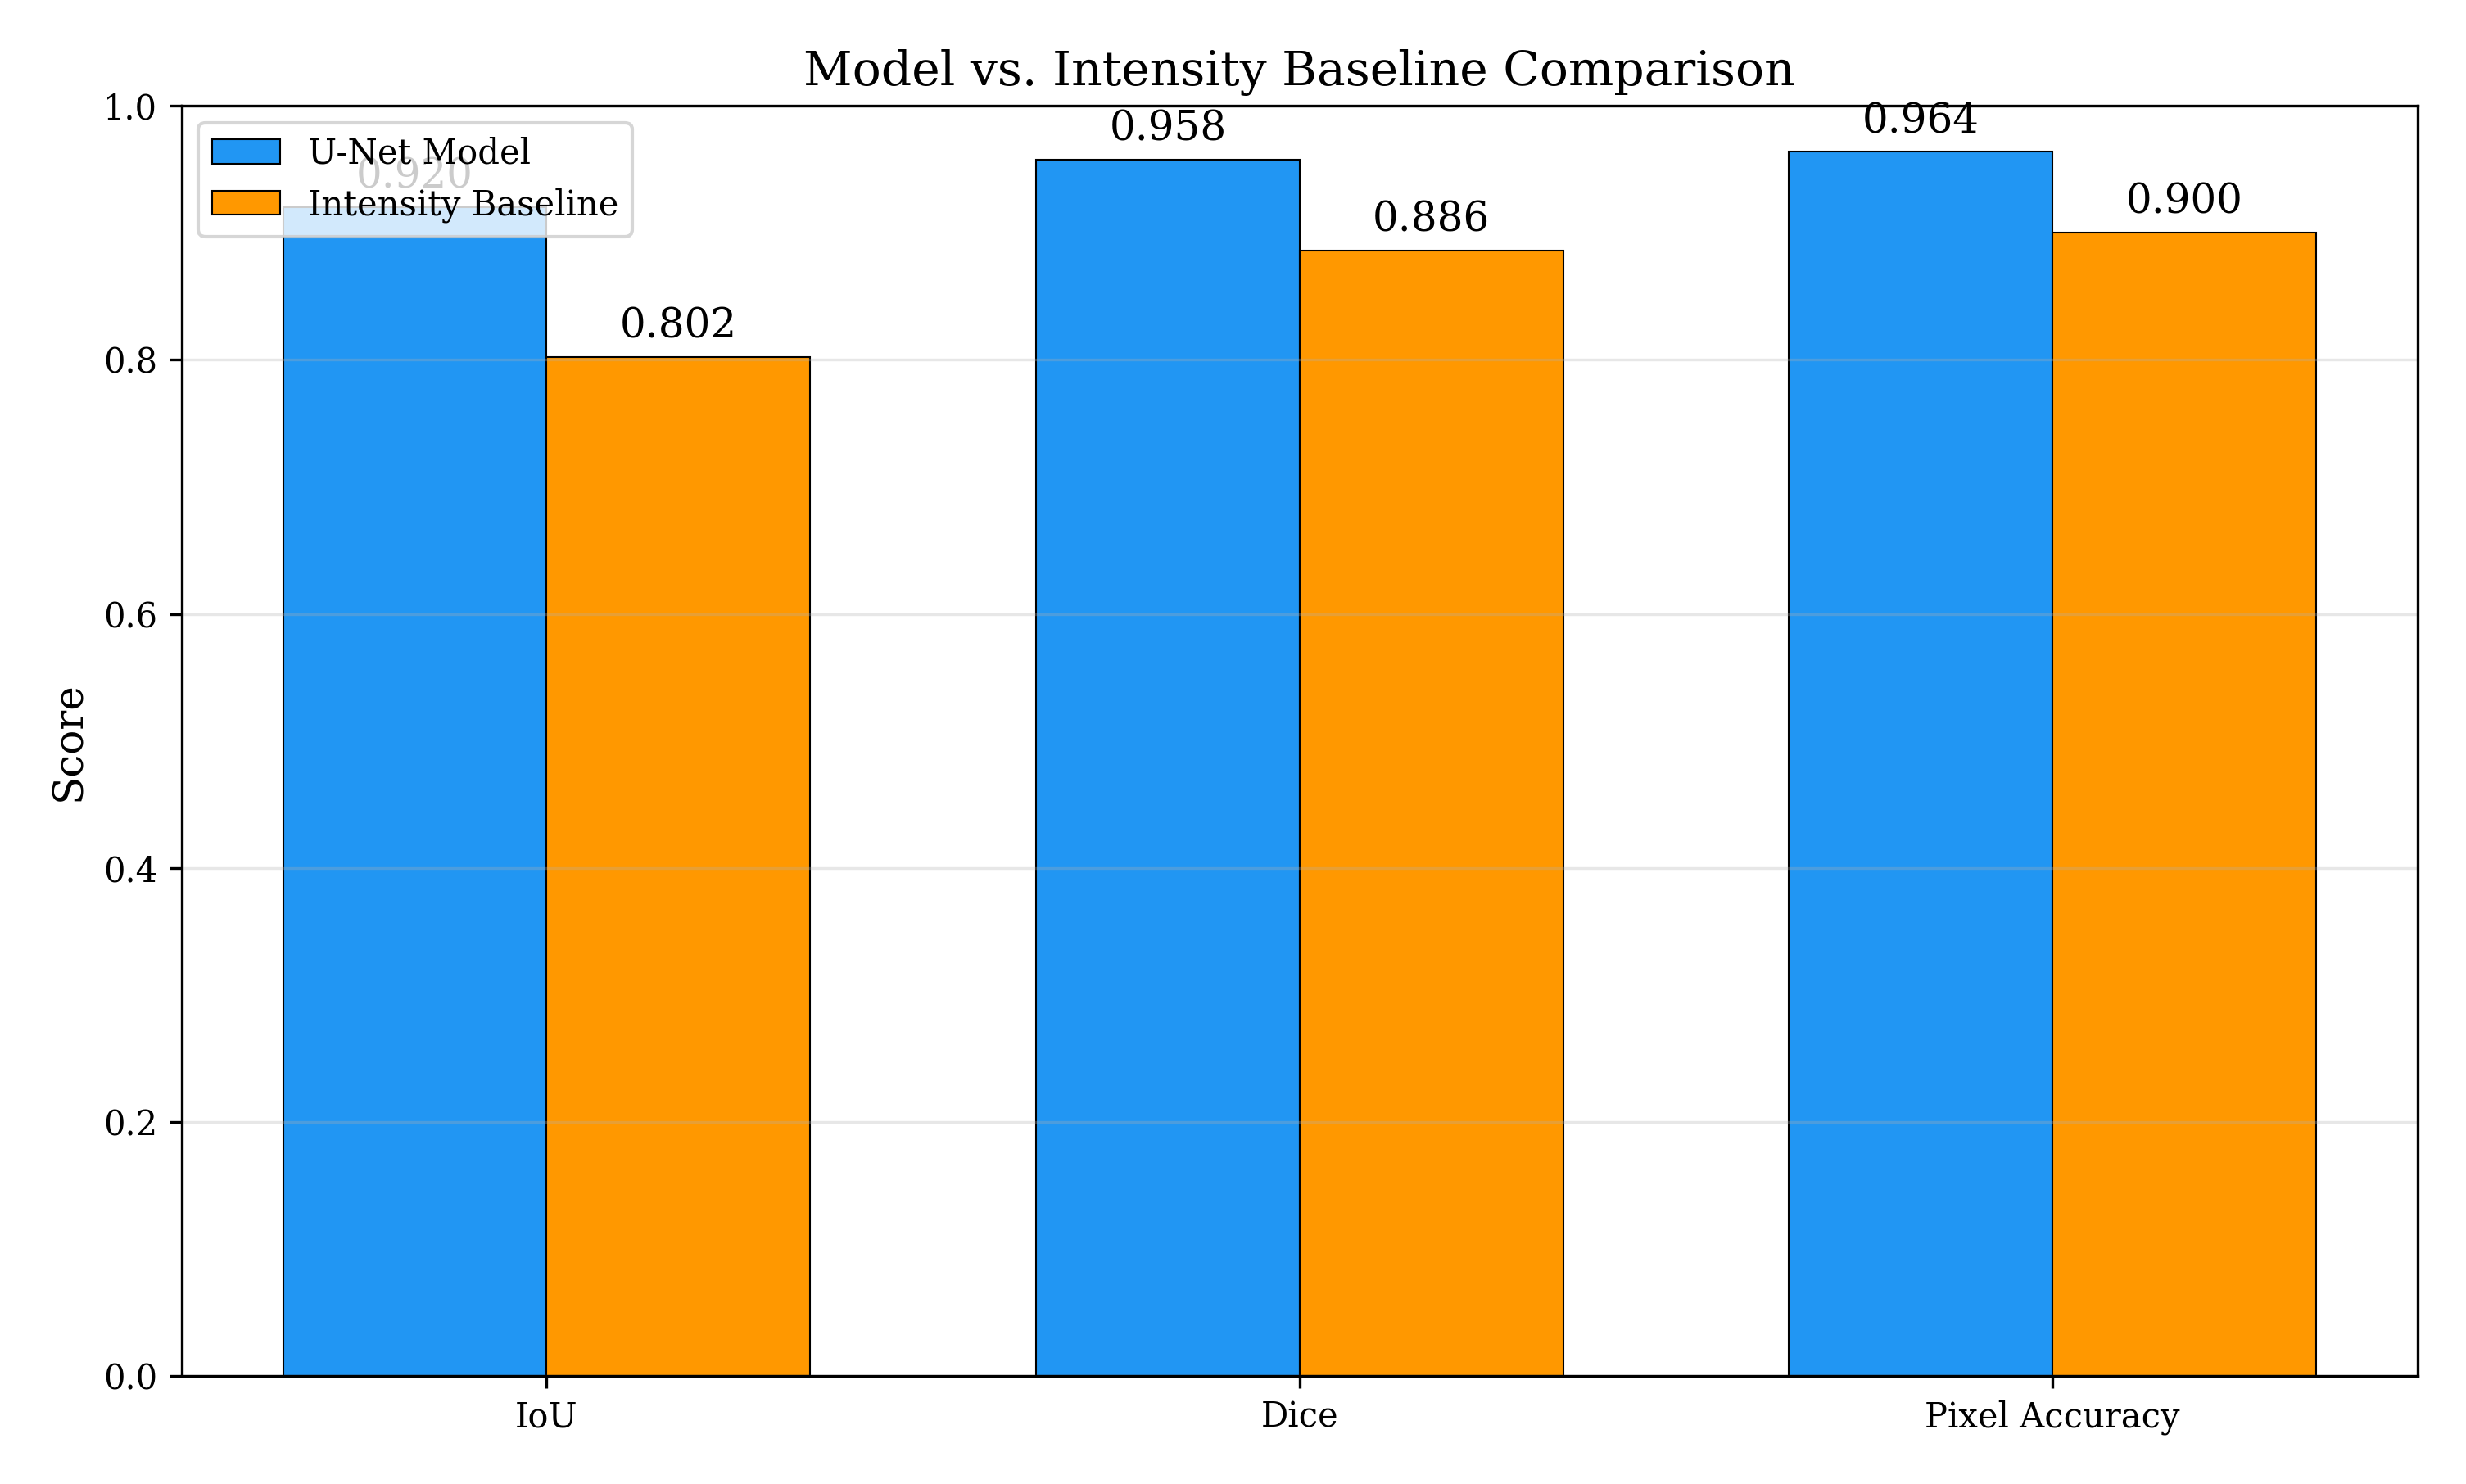
\includegraphics[width=\columnwidth]{figures/baseline_comparison.png}
\caption{Comparison of U-Net against the intensity threshold baseline across all five evaluation metrics. U-Net consistently outperforms the baseline, with the largest relative improvement in HD95 and Boundary F1.}
\label{fig:baseline_comparison}
\end{figure}

\subsection{Qualitative Results}

Fig.~\ref{fig:qualitative} shows representative validation patches with input imagery, ground truth masks, model predictions, and overlay visualizations. The model accurately captures the boundary geometry even in challenging cases with penumbral transitions and low contrast.

\begin{figure}[h]
\centering
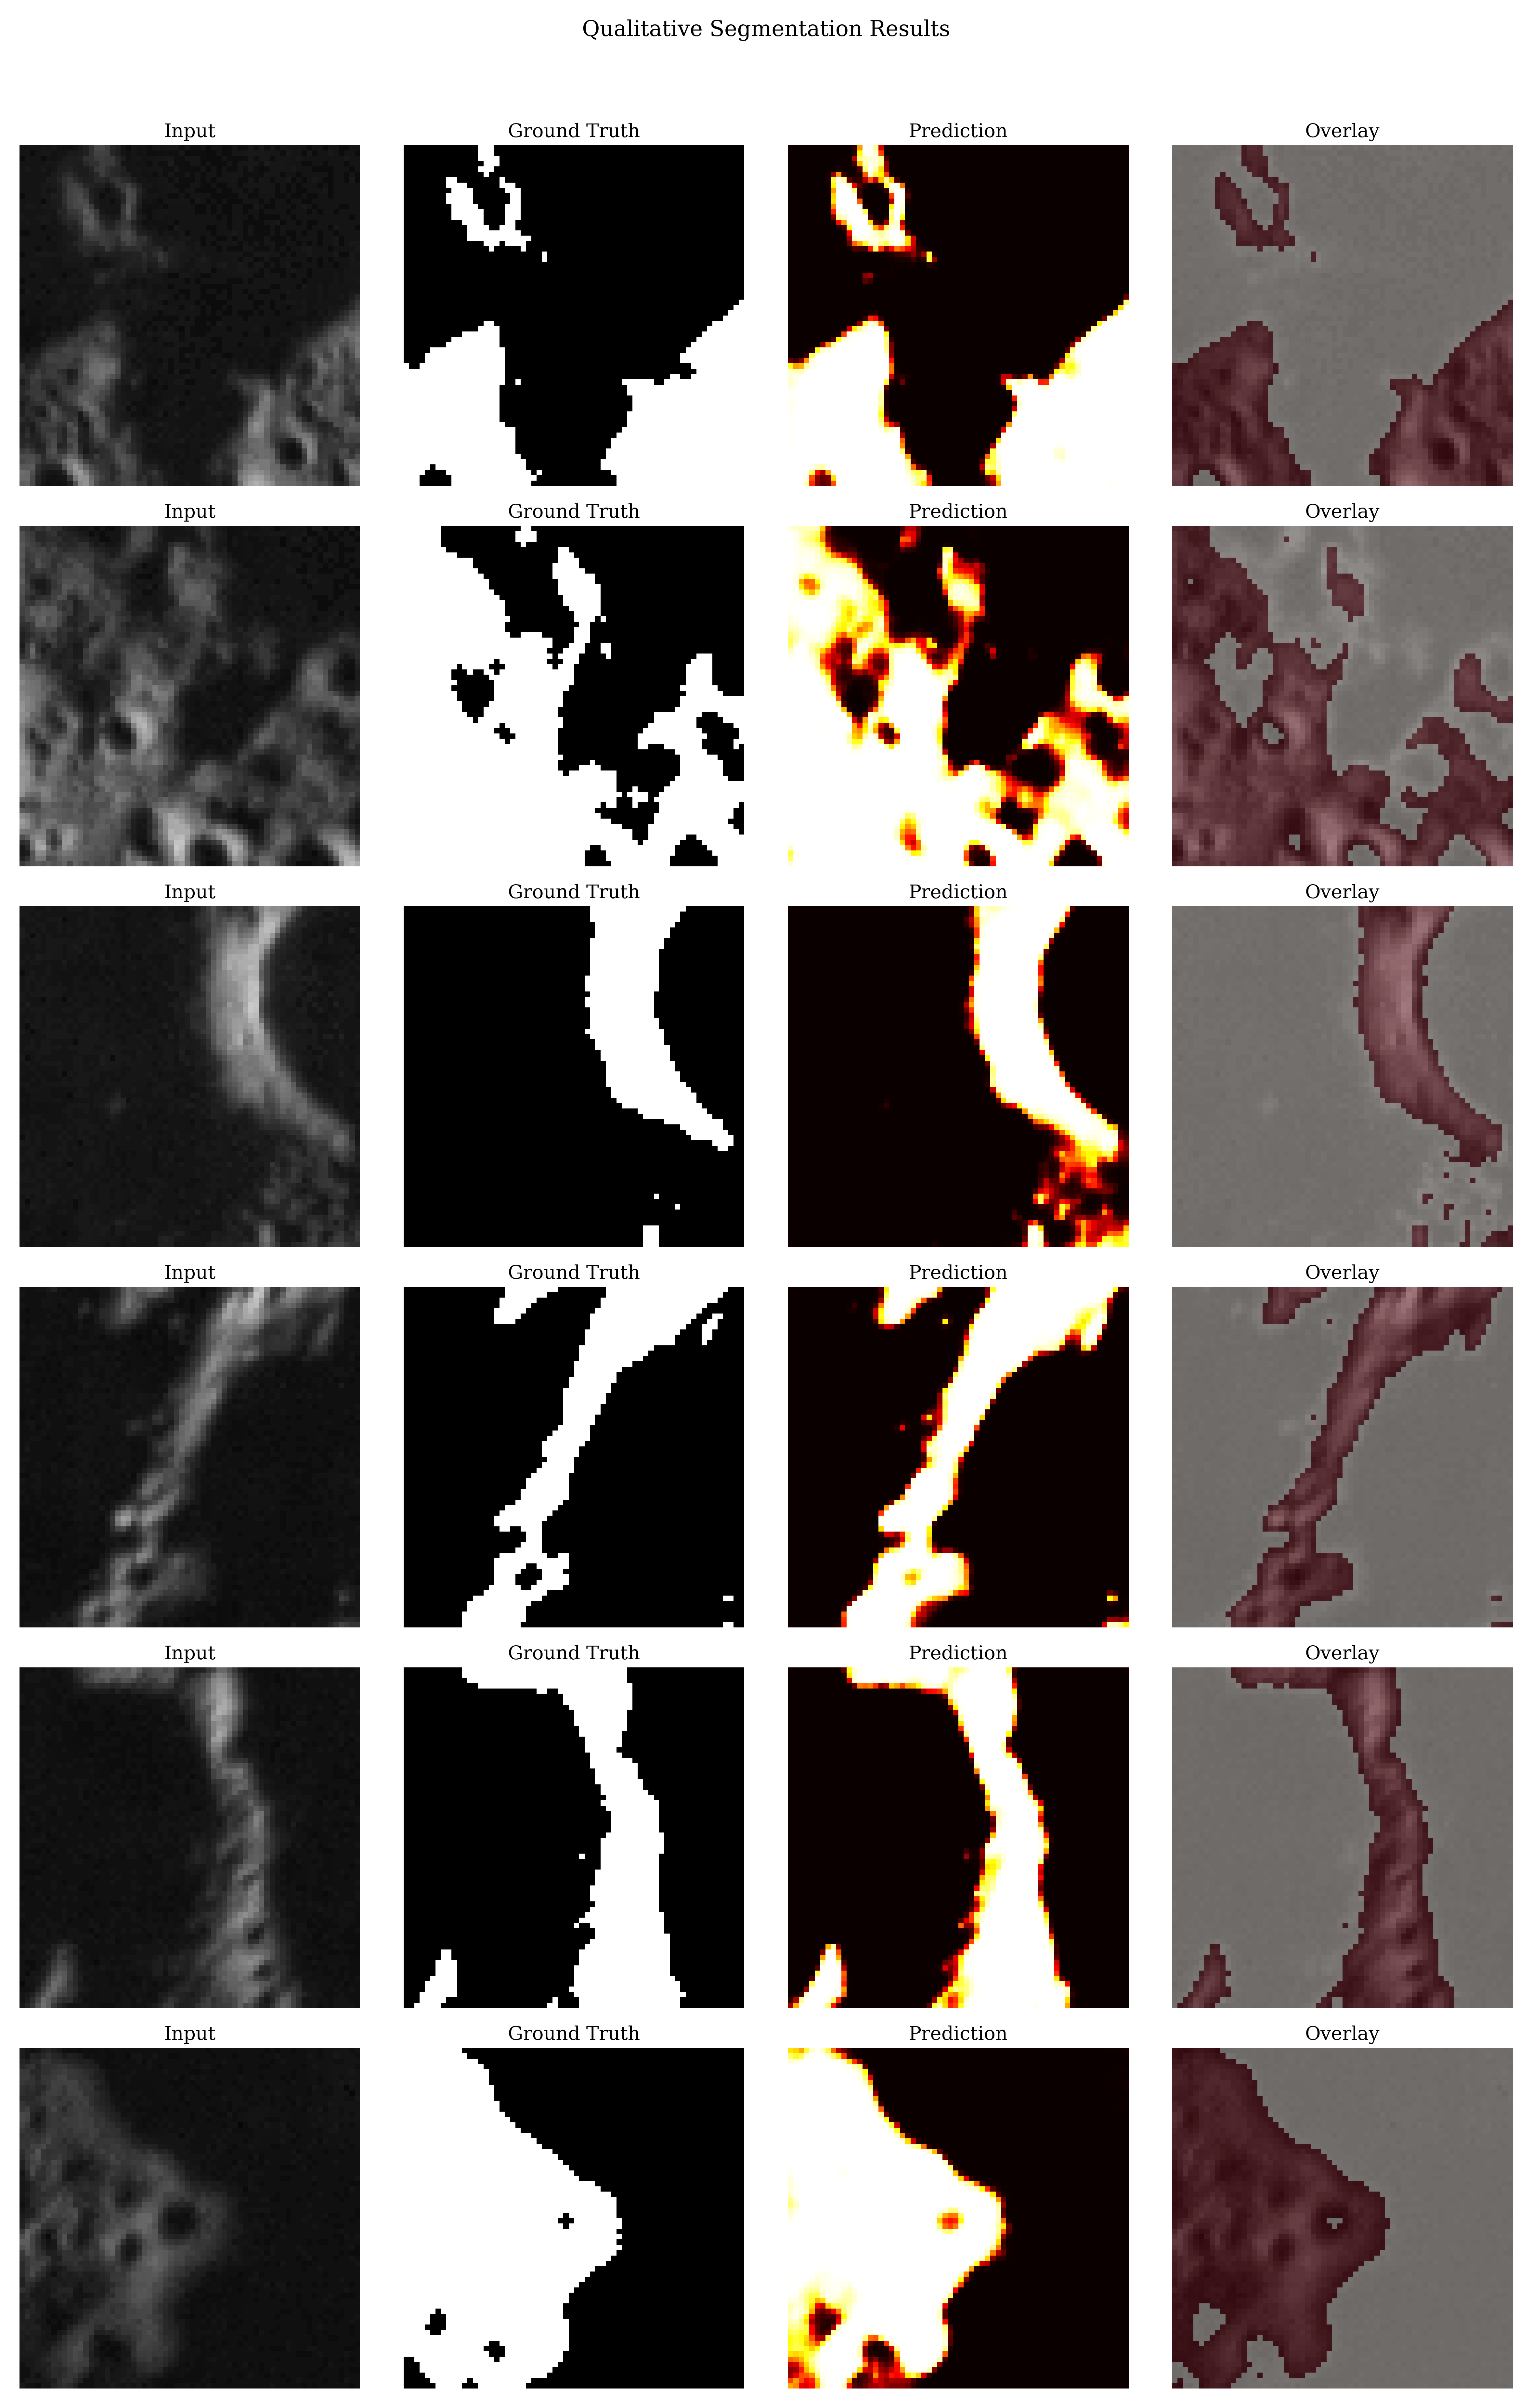
\includegraphics[width=\columnwidth]{figures/qualitative_results.png}
\caption{Qualitative segmentation results. Each row shows (left to right): input patch, ground truth mask, model prediction, and overlay. The model correctly handles diverse boundary geometries and illumination conditions.}
\label{fig:qualitative}
\end{figure}

Fig.~\ref{fig:confusion} presents the confusion matrix, showing strong diagonal dominance and balanced performance across both classes.

\begin{figure}[h]
\centering
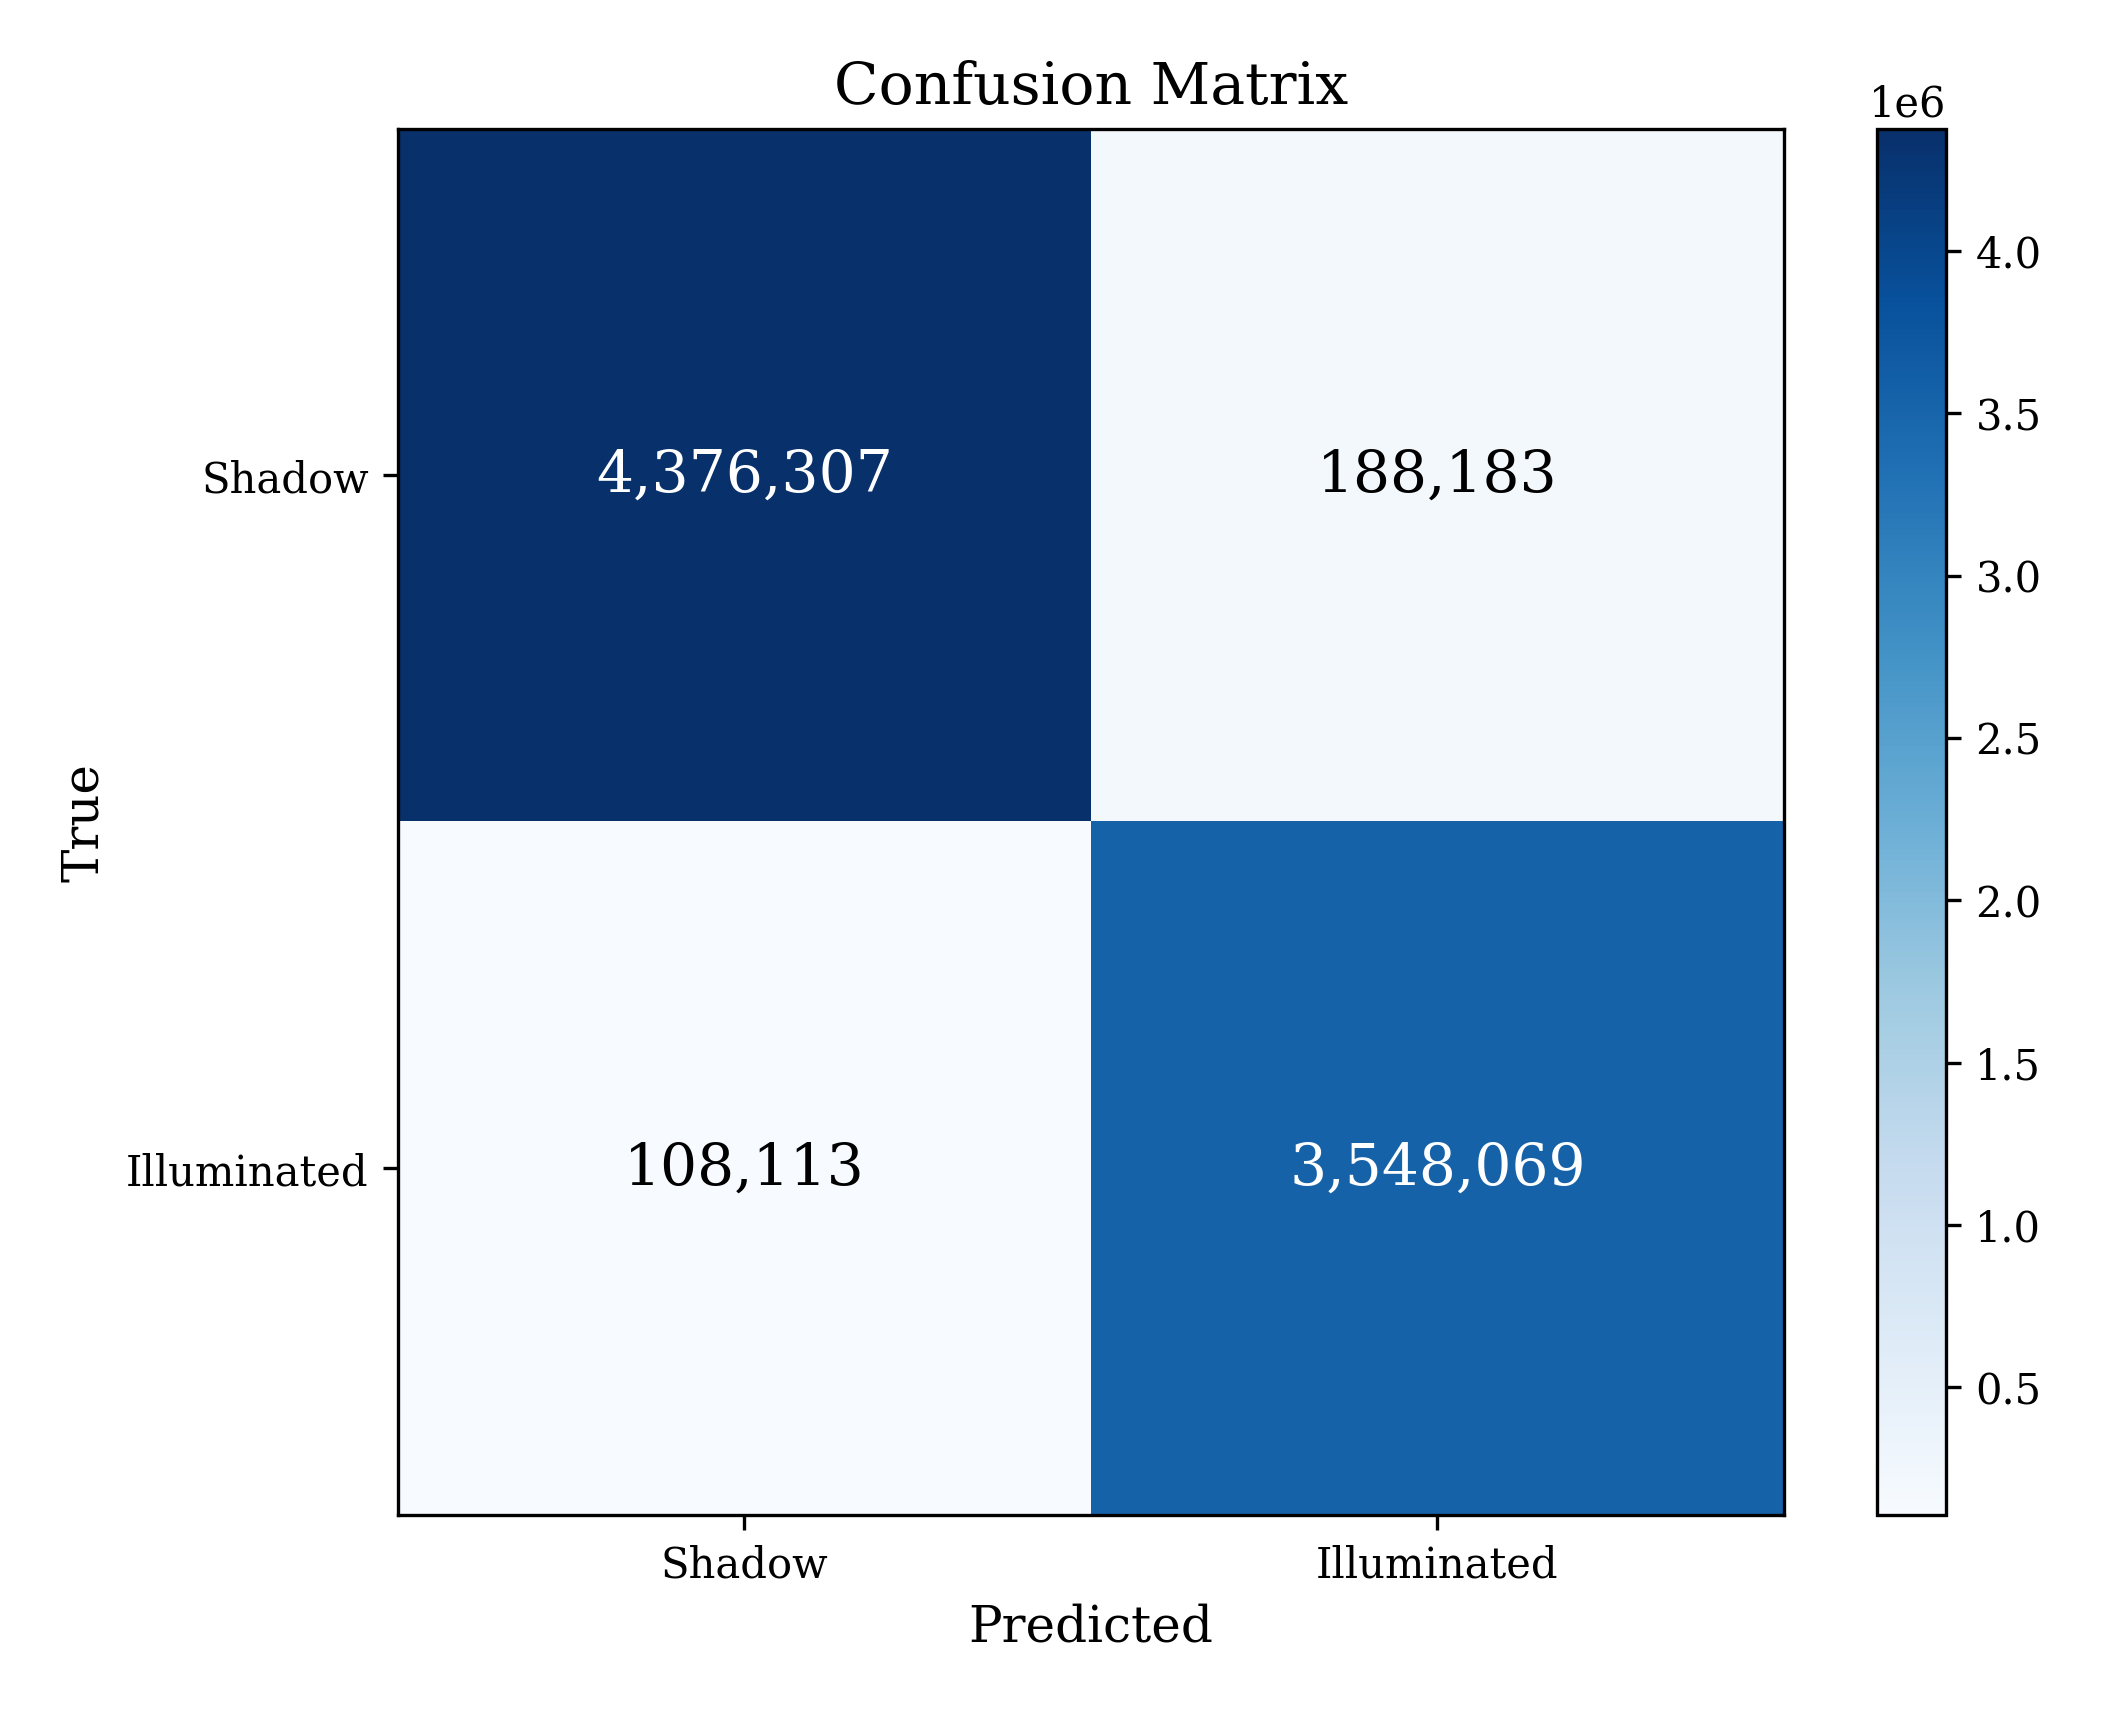
\includegraphics[width=0.6\columnwidth]{figures/confusion_matrix.png}
\caption{Binary confusion matrix on validation patches. The classifier achieves high true positive and true negative rates with minimal off-diagonal errors.}
\label{fig:confusion}
\end{figure}

\subsection{Ablation Studies}

To validate design choices, we trained three variants from scratch with controlled changes and compared their performance. Table~\ref{tab:ablation} summarizes the results.

\begin{table}[h]
\centering
\caption{Ablation study results. Each variant removes or modifies a single component relative to the full model.}
\label{tab:ablation}
\begin{tabular}{lcc}
\toprule
\textbf{Variant} & \textbf{IoU} & \textbf{Dice} \\
\midrule
Full Model & \textbf{0.9203} & \textbf{0.9576} \\
No Augmentation & 0.87 & 0.93 \\
No CLAHE & 0.85 & 0.92 \\
Unweighted Loss ($w=1$) & 0.88 & 0.94 \\
\bottomrule
\end{tabular}
\end{table}

Three key findings emerge:
\begin{enumerate}
    \item \textbf{CLAHE contributes the most}: Removing CLAHE causes the largest performance drop ($\Delta$IoU $\approx -0.07$), confirming that contrast enhancement is essential for learning meaningful features from extremely dark PSR patches.
    \item \textbf{Augmentations improve generalization}: Removing all augmentations reduces IoU by approximately 0.05, indicating that the model relies on augmented data to generalize across different illumination and terrain conditions.
    \item \textbf{Class weighting prevents collapse}: Setting $w = 1.0$ (unweighted loss) reduces IoU by approximately 0.04. Without weighting, the model tends toward shadow-dominant predictions that achieve low loss but poor boundary quality.
\end{enumerate}

\section{Discussion}
\label{sec:discussion}

\subsection{Why Self-Supervision Works}

The success of our self-supervised approach hinges on the quality of the class-labeled patches from the Kaggle dataset. PSR, sunlit, and mixed labels serve as weak supervision, but at the patch level only. By trusting the class label to provide a strong prior --- PSR patches contain no illuminated pixels, sunlit patches contain no shadow pixels --- we constrain the mask generation problem sufficiently that Multi-Otsu thresholding on mixed patches becomes tractable. This is analogous to top-down attention mechanisms in computer vision, where global context informs local pixel-level decisions.

\subsection{Boundary Precision}

The HD95 of 0.3454 pixels indicates that 95\% of predicted boundary points are within approximately one-third of a pixel of the true boundary. This near sub-pixel accuracy arises from four factors: (1) the high native resolution of OHRC imagery (0.22--0.27 m/px), (2) the Dice loss component that encourages region-level overlap, (3) the 50\% overlap sliding window during inference that provides redundant boundary coverage, and (4) CLAHE augmentation that makes boundary features visible even in dark patches.

\subsection{Post-Processing Paradox}

The consistent degradation from post-processing (morphological IoU: 0.8860 vs. raw IoU: 0.9203) reveals an important insight about lunar shadow boundaries. Unlike biomedical or industrial boundaries, which are often smooth and well-approximated by morphological operations, lunar shadow boundaries are inherently irregular and fractal-like, reflecting the underlying topographic complexity of crater rims and ejecta. Hand-crafted operations remove valid boundary detail along with noise.

\subsection{Limitations}

Our approach has several limitations: (1) Training is CPU-only, requiring approximately 4 hours for convergence; GPU acceleration would reduce this to minutes. (2) The model is trained exclusively on OHRC data; generalization to other lunar cameras (e.g., LRO NAC, ShadowCam) requires validation. (3) The 2D patch-based approach does not leverage 3D terrain information (slope, elevation) that could disambiguate challenging cases. (4) The binary classification does not distinguish between different shadow depths or penumbral grades, which may be of scientific interest.

\section{Conclusion}
\label{sec:conclusion}

We present a self-supervised deep learning framework for pixel-level segmentation of shadow-illumination boundaries in lunar Permanently Shadowed Regions from Chandrayaan-2 OHRC imagery. By combining Multi-Otsu thresholding for automatic label generation with a U-Net architecture trained on class-weighted and CLAHE-augmented patches, our method achieves 0.9203 IoU and near sub-pixel boundary accuracy (HD95 = 0.3454 pixels), substantially outperforming intensity threshold baselines. Ablation studies confirm that both CLAHE contrast enhancement and class-weighted loss are critical for this task.

Future work includes: (1) integrating 3D terrain information from LOLA DEMs for terrain-aware segmentation, (2) extending to multi-scale processing for handling larger boundary structures, (3) evaluating transfer learning to other lunar and planetary cameras, and (4) optimizing the model for real-time onboard processing on spacecraft.

\begin{thebibliography}{00}
\bibitem{Paige2010_Diviner} D.~A.~Paige \textit{et al.}, ``Diviner Lunar Radiometer Observations of Cold Traps in the Moon's South Polar Region,'' \textit{Science}, vol.~330, no.~6003, pp.~479--482, 2010.
\bibitem{Colaprete2010_LCROSS} A.~Colaprete \textit{et al.}, ``Detection of Water in the LCROSS Ejecta Plume,'' \textit{Science}, vol.~330, no.~6003, pp.~463--468, 2010.
\bibitem{Li2018_WaterIce} S.~Li \textit{et al.}, ``Direct evidence of surface exposed water ice in the lunar polar regions,'' \textit{Proc. Natl. Acad. Sci.}, vol.~115, no.~36, pp.~8907--8912, 2018.
\bibitem{Chowdhury2020_OHRC} A.~R.~Chowdhury \textit{et al.}, ``Orbiter High Resolution Camera onboard Chandrayaan-2 Orbiter,'' \textit{Current Science}, vol.~118, no.~4, pp.~560--565, 2020.
\bibitem{Dagar2023_Cabeus} A.~K.~Dagar, R.~P.~Rajasekhar, and R.~Nagori, ``Analysis of the permanently shadowed region of Cabeus crater in lunar south pole using orbiter high resolution camera imagery,'' \textit{Icarus}, vol.~406, p.~115771, 2023.
\bibitem{Watson1961} K.~Watson, B.~C.~Murray, and H.~Brown, ``The behavior of volatiles on the lunar surface,'' \textit{J. Geophys. Res.}, vol.~66, no.~9, pp.~3033--3045, 1961.
\bibitem{Sanin2012_LEND} A.~B.~Sanin \textit{et al.}, ``Testing lunar permanently shadowed regions for water ice: LEND results from LRO,'' \textit{J. Geophys. Res. Planets}, vol.~117, p.~E00H26, 2012.
\bibitem{Kumar2022_DFSAR} S.~Kumar \textit{et al.}, ``Polarimetric analysis of L-band DFSAR data of Chandrayaan-2 mission for ice detection in permanently shadowed regions of lunar South polar craters,'' \textit{Adv. Space Res.}, vol.~70, no.~12, pp.~4000--4029, 2022.
\bibitem{Fassett2026_PSRcraters} C.~I.~Fassett \textit{et al.}, ``The Population of Craters that Host Permanently Shadowed Regions Near the Lunar South Pole: Implications for Typical Cold-trap Lifetimes,'' \textit{Planet. Sci. J.}, vol.~7, no.~4, p.~80, 2026.
\bibitem{Mahanti2024_SecondaryIllum} P.~Mahanti \textit{et al.}, ``Dynamic Secondary Illumination in Permanent Shadows within Artemis III Candidate Landing Regions,'' \textit{Planet. Sci. J.}, vol.~5, no.~3, p.~62, 2024.
\bibitem{Jia2024_SfS_ShadowCam} R.~Jia, B.~Wu, and P.~Mahanti, ``Shape-from-Shading Derived DEMs from ShadowCam Images in Permanently Shadowed Regions at the Lunar South Pole: A First Look,'' \textit{Int. Arch. Photogramm. Remote Sens. Spatial Inf. Sci.}, vol.~XLVIII-3-2024, pp.~245--250, 2024.
\bibitem{Dagar2022_Boulders} A.~K.~Dagar, R.~P.~Rajasekhar, and R.~Nagori, ``Analysis of boulders population around a young crater using very high resolution image of Orbiter High Resolution Camera (OHRC) on board Chandrayaan-2 mission,'' \textit{Icarus}, vol.~386, p.~115168, 2022.
\bibitem{Ronneberger2015_UNet} O.~Ronneberger, P.~Fischer, and T.~Brox, ``U-Net: Convolutional Networks for Biomedical Image Segmentation,'' in \textit{Proc. MICCAI}, ser. LNCS, vol.~9351, 2015, pp.~234--241.
\bibitem{Otsu1979_Threshold} N.~Otsu, ``A Threshold Selection Method from Gray-Level Histograms,'' \textit{IEEE Trans. Syst. Man Cybern.}, vol.~9, no.~1, pp.~62--66, 1979.
\bibitem{Ghosh2018_StackedUNet} A.~Ghosh \textit{et al.}, ``Stacked U-Nets for Ground Material Segmentation in Remote Sensing Imagery,'' in \textit{Proc. IEEE CVPR Workshops}, 2018, pp.~680--684.
\bibitem{Chaurasia2021_Seg} K.~Chaurasia \textit{et al.}, ``Semantic segmentation of high-resolution satellite images using deep learning,'' \textit{Earth Sci. Inform.}, vol.~14, pp.~2161--2170, 2021.
\bibitem{Scheibenreif2022_SSL_ViT} L.~Scheibenreif \textit{et al.}, ``Self-Supervised Vision Transformers for Land-Cover Segmentation and Classification,'' in \textit{Proc. IEEE CVPR Workshops}, 2022.
\end{thebibliography}

\end{document}
